\section{Dữ liệu ảnh: Phân loại cảnh quan tự nhiên (Intel Image)}
\label{sec:image}

\subsection{Dữ liệu và Khám phá đặc trưng thị giác (EDA)}
Bài toán sử dụng bộ \textit{Intel Image Classification} \cite{bansal2019intel} gồm \textbf{17.034 ảnh RGB} thuộc \textbf{6 lớp} (\textit{buildings, forest, glacier, mountain, sea, street}), chia sẵn thành 14.034 ảnh Train và 3.000 ảnh Test độc lập. Kiểm tra toàn vẹn cho thấy 0 tệp lỗi, 100\% ảnh ở chế độ 3 kênh màu RGB, đa số kích thước $150\times 150$ px (đạt chuẩn $\ge 128$ px của Assignment v4; một số ít ảnh có chiều cao nhỏ hơn được chuẩn hóa bằng resize/padding).

\begin{figure}[H]
  \centering
  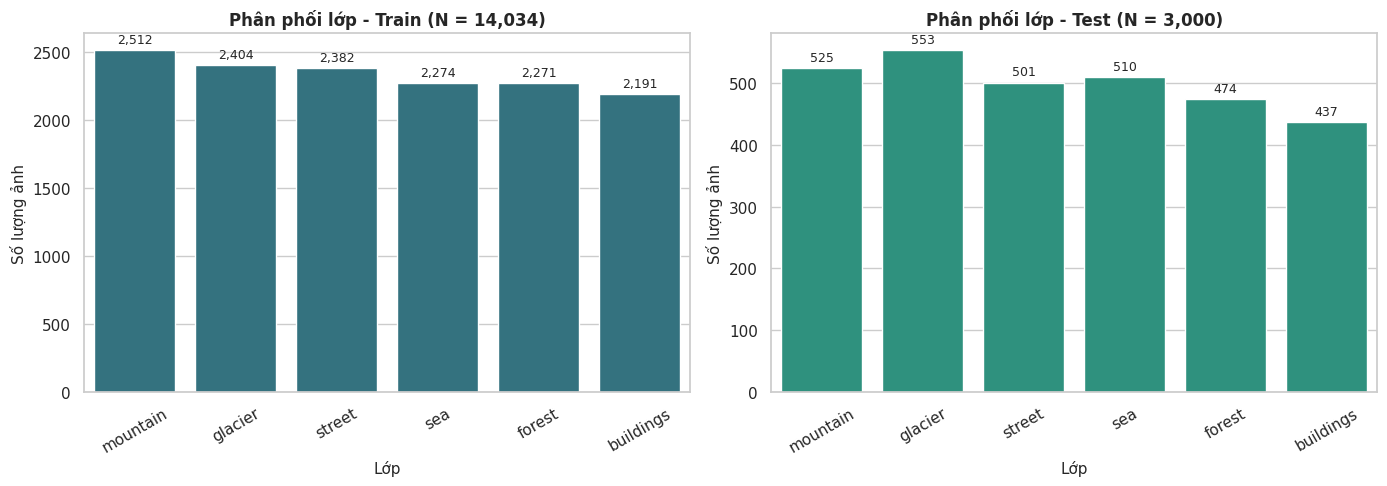
\includegraphics[width=0.86\linewidth]{image/c11_f0.png}
  \caption{Phân phối số lượng ảnh theo 6 lớp trên tập Train (14.034 ảnh) và Test (3.000 ảnh): các lớp tương đối cân bằng (14,57\% -- 18,43\%), không cần áp dụng kỹ thuật cân bằng lớp nhân tạo.}
  \label{fig:img_dist}
\end{figure}

Nhóm tách tập Train ban đầu theo tỷ lệ phân tầng (\textit{Stratified Split}) thành \textbf{Train (85\% -- 11.928 ảnh)} và \textbf{Validation (15\% -- 2.106 ảnh)}, giữ nguyên \textbf{Test (3.000 ảnh)} độc lập. Trực quan hóa bằng t-SNE trên 24 đặc trưng histogram màu RGB toàn cục (\Cref{fig:img_tsne}) cho thấy \textit{forest} tách biệt khá rõ nhờ sắc xanh lá, trong khi \textit{glacier} -- \textit{mountain} và \textit{buildings} -- \textit{street} chồng lấn mạnh do chia sẻ tông màu và cấu trúc nền.

\begin{figure}[H]
  \centering
  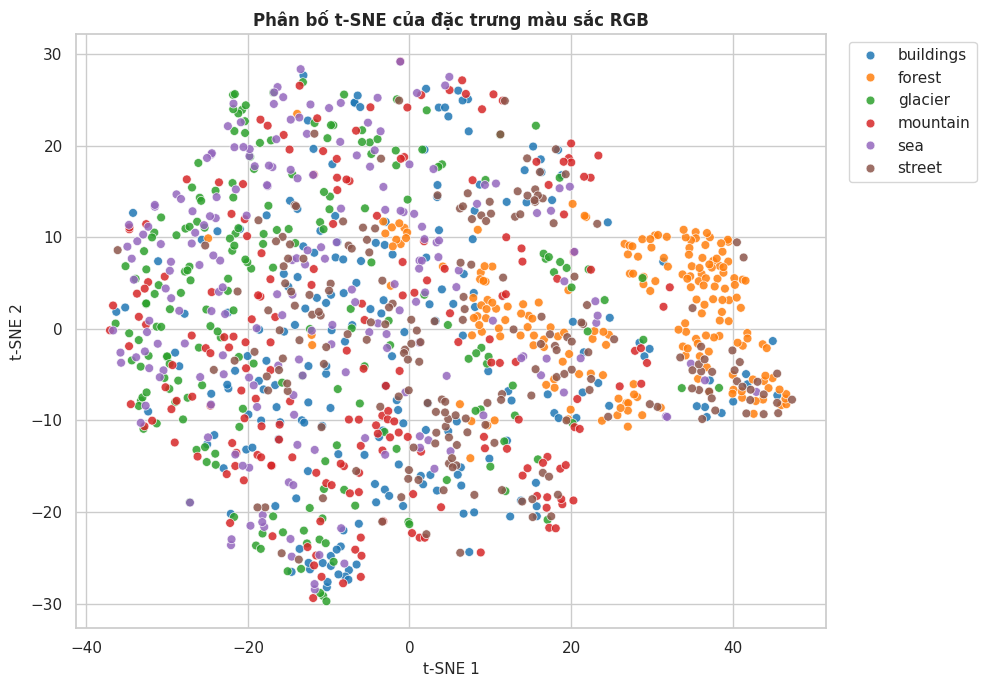
\includegraphics[width=0.84\linewidth]{image/c25_f0.png}
  \caption{Trực quan hóa t-SNE từ đặc trưng màu RGB toàn cục (1.200 mẫu): đặc trưng màu thủ công phân tách tốt \textit{forest}, nhưng chồng lấn nặng giữa \textit{mountain}--\textit{glacier} và \textit{buildings}--\textit{street}, chứng minh cần đặc trưng không gian sâu.}
  \label{fig:img_tsne}
\end{figure}

\subsection{Thiết kế thực nghiệm và Pipeline huấn luyện}
Nhóm sử dụng chuẩn \textit{Data Augmentation} trên tập Train (RandomResizedCrop/Resize, HorizontalFlip, ColorJitter nhẹ và chuẩn hóa theo thống kê ImageNet) với \texttt{batch\_size = 64} trên GPU Tesla T4. Bảy cấu hình mô hình thuộc 4 hệ quy chiếu được đối chiếu công bằng trên cùng tập Test 3.000 ảnh:
\begin{enumerate}[leftmargin=*]
  \item \textbf{Huấn luyện từ đầu (\textit{From Scratch}):} \texttt{SimpleBaselineCNN} (0,42M tham số, 10 epochs) và \texttt{ResNet-18 Scratch} (11,18M tham số, 12 epochs).
  \item \textbf{Pretrained Feature Extractor (\textit{Linear Probe}):} \texttt{ResNet-18} đóng băng backbone, chỉ huấn luyện lớp phân loại cuối (3.078 tham số, 5 epochs).
  \item \textbf{Pretrained Fine-tuning:} \texttt{ResNet-18} mở khóa \texttt{layer4+fc} (8,40M tham số, 6 epochs) và \texttt{ViT-B/16} (14,18M tham số huấn luyện / 85,80M tổng, 6 epochs).
  \item \textbf{Zero-shot Foundation Model:} \texttt{CLIP ViT-B/32} \cite{radford2021learning} (không huấn luyện, 0 tham số cập nhật) với cấu hình Basic và Prompt Ensemble.
\end{enumerate}

\subsection{Bảng đối chiếu Benchmark và Đánh đổi kỹ thuật}

\Cref{tab:img_benchmark} và \Cref{fig:img_benchmark} tổng hợp toàn diện độ chính xác, tốc độ suy luận và tài nguyên VRAM của cả 7 mô hình trên tập Test.

\begin{table}[H]
  \centering
  \caption{Bảng đối chiếu hiệu năng và chi phí kỹ thuật của 7 mô hình trên tập Test độc lập (3.000 ảnh).}
  \label{tab:img_benchmark}
  \resizebox{\linewidth}{!}{%
  \begin{tabular}{l l r r r r r r}
    \toprule
    \textbf{Mô hình} & \textbf{Phương pháp} & \textbf{Trainable} & \textbf{Train (s)} & \textbf{VRAM (MB)} & \textbf{Latency (ms)} & \textbf{Test Acc (\%)} & \textbf{Macro-F1 (\%)} \\
    \midrule
    ViT-B/16 (Fine-tune) & Vision Transformer & 14,18M & 1262,8 & 2276,6 & 11,20 & \textbf{94,87} & \textbf{94,98} \\
    ResNet-18 (Fine-tune) & Partial Fine-tune & 8,40M & 439,2 & 753,4 & 3,42 & 93,90 & 93,99 \\
    CLIP ViT-B/32 (Ensemble) & Zero-shot VLM & 0 & 0,0 & 1441,4 & 5,17 & 93,43 & 93,58 \\
    CLIP ViT-B/32 (Basic) & Zero-shot VLM & 0 & 0,0 & 1441,4 & 5,08 & 93,00 & 93,10 \\
    ResNet-18 (Linear Probe) & Frozen Backbone & 3.078 & 391,7 & 606,9 & 3,00 & 89,87 & 90,02 \\
    ResNet-18 (Scratch) & From Scratch & 11,18M & 577,9 & 909,3 & 2,02 & 89,40 & 89,50 \\
    SimpleBaselineCNN & From Scratch & 0,42M & 458,3 & 1048,2 & \textbf{1,76} & 85,80 & 85,87 \\
    \bottomrule
  \end{tabular}%
  }
\end{table}

\begin{figure}[H]
  \centering
  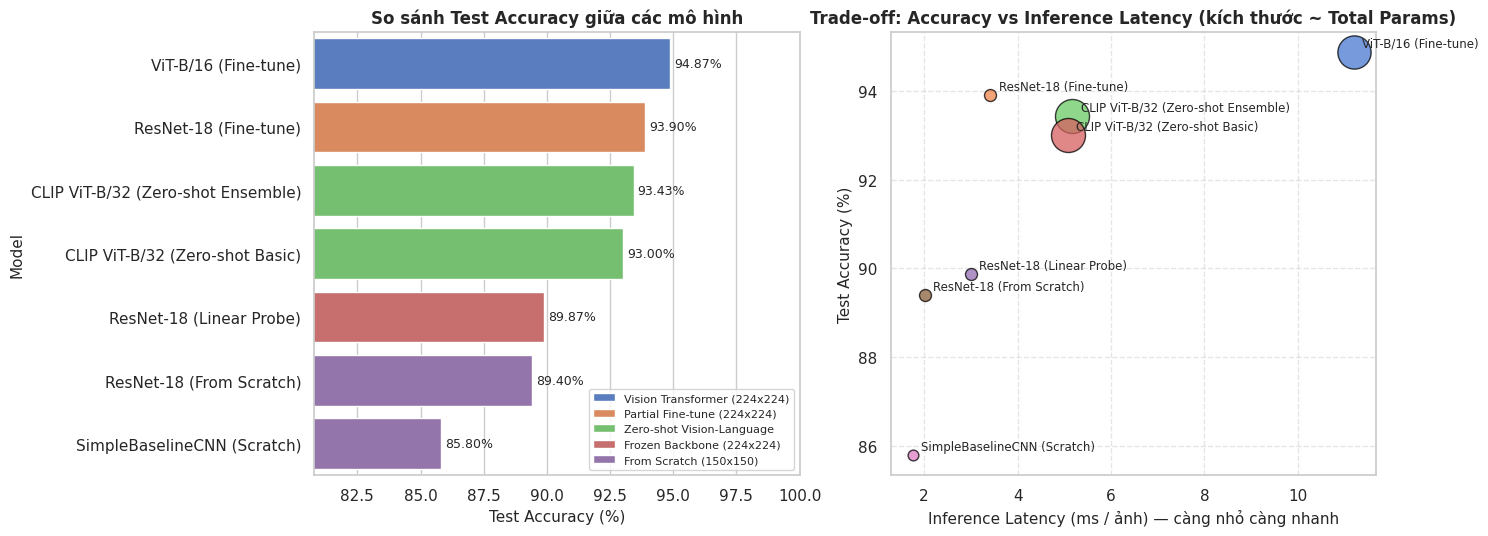
\includegraphics[width=0.90\linewidth]{image/c53_f0.png}
  \caption{Đối chiếu Test Accuracy, Macro-F1 và độ trễ suy luận giữa 7 mô hình: \textit{ViT-B/16 (Fine-tune)} đạt Accuracy cao nhất (94,87\%) nhưng tốn 11,20 ms/ảnh; \textit{ResNet-18 (Fine-tune)} cân bằng tối ưu nhất (93,90\% với chỉ 3,42 ms/ảnh và 753,4 MB VRAM).}
  \label{fig:img_benchmark}
\end{figure}

Từ kết quả thực nghiệm rút ra 3 nhận định cốt lõi:
\begin{itemize}[leftmargin=*]
  \item \textbf{Transfer Learning vượt trội From Scratch:} \textit{ResNet-18 (Fine-tune)} đạt 93,90\%, cao hơn +4,50 điểm \% so với \textit{ResNet-18 (Scratch)} (89,40\%) và +8,10 điểm \% so với \textit{SimpleBaselineCNN} (85,80\%), đồng thời hội tụ nhanh hơn (6 epochs vs 12 epochs).
  \item \textbf{Sức mạnh của Zero-shot CLIP:} Không cần bất kỳ mẫu huấn luyện nào, \textit{CLIP ViT-B/32 (Ensemble)} đạt tới \textbf{93,43\%}, vượt qua cả \textit{ResNet-18 Linear Probe} (89,87\%). Đặc biệt, trên 183 ca \textit{ResNet-18 (Fine-tune)} đoán sai, \textit{CLIP} đoán đúng lại tới \textbf{93/183 ca (50,8\%)} và \textit{ViT-B/16} đoán đúng lại \textbf{80/183 ca (43,7\%)}.
  \item \textbf{Đánh đổi chi phí -- hiệu năng:} \textit{ViT-B/16} đạt đỉnh 94,87\% nhưng có độ trễ gấp 3,27 lần và VRAM gấp 3,02 lần so với \textit{ResNet-18 (Fine-tune)}.
\end{itemize}

\subsection{Phân tích lỗi và Minh bạch hóa bằng Grad-CAM (XAI)}
Ma trận nhầm lẫn (\Cref{fig:img_cm}) và danh sách mẫu sai (\Cref{fig:img_errors}) xác nhận đúng dự báo từ bước EDA: lỗi của \textit{ResNet-18 (Fine-tune)} tập trung chủ yếu ở hai cặp lớp giao thoa tự nhiên là \textit{mountain} $\leftrightarrow$ \textit{glacier} (45 ca mountain nhầm thành glacier [8,57\%] và 39 ca ngược lại [7,05\%]) và \textit{street} $\leftrightarrow$ \textit{buildings} (31 ca street nhầm thành buildings [6,19\%] và 24 ca ngược lại [5,49\%]). Trong khi đó, \textit{forest} (F1 = 99,26\%) và \textit{sea} (F1 = 96,82\%) đạt độ chính xác gần như tuyệt đối.

\begin{figure}[H]
  \centering
  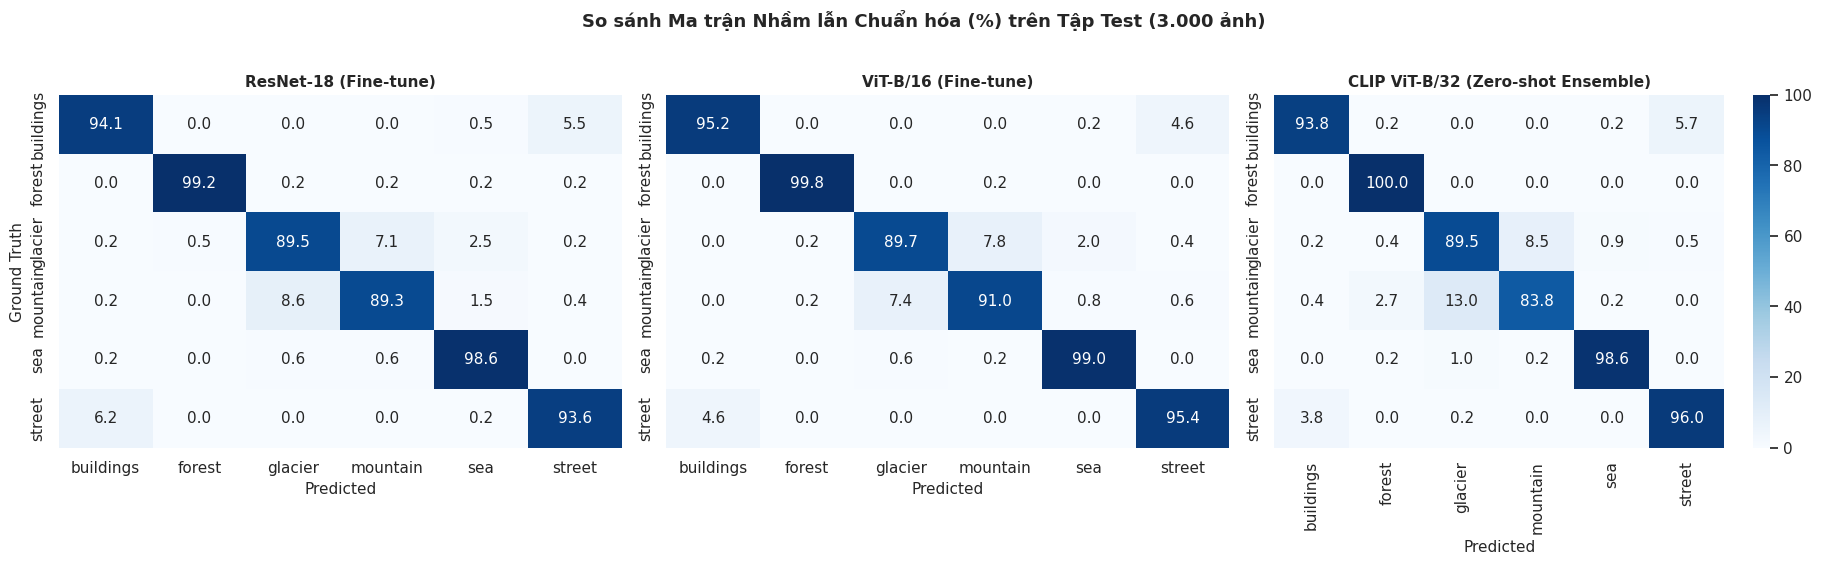
\includegraphics[width=0.90\linewidth]{image/c55_f0.png}
  \caption{Ma trận nhầm lẫn và F1-Score theo từng lớp: \textit{forest} đạt F1 99,26\% (ResNet-18 Fine-tune) và 99,68\% (ViT-B/16), trong khi phần lớn sai số nằm ở cặp \textit{mountain}--\textit{glacier} và \textit{buildings}--\textit{street}.}
  \label{fig:img_cm}
\end{figure}

\begin{figure}[H]
  \centering
  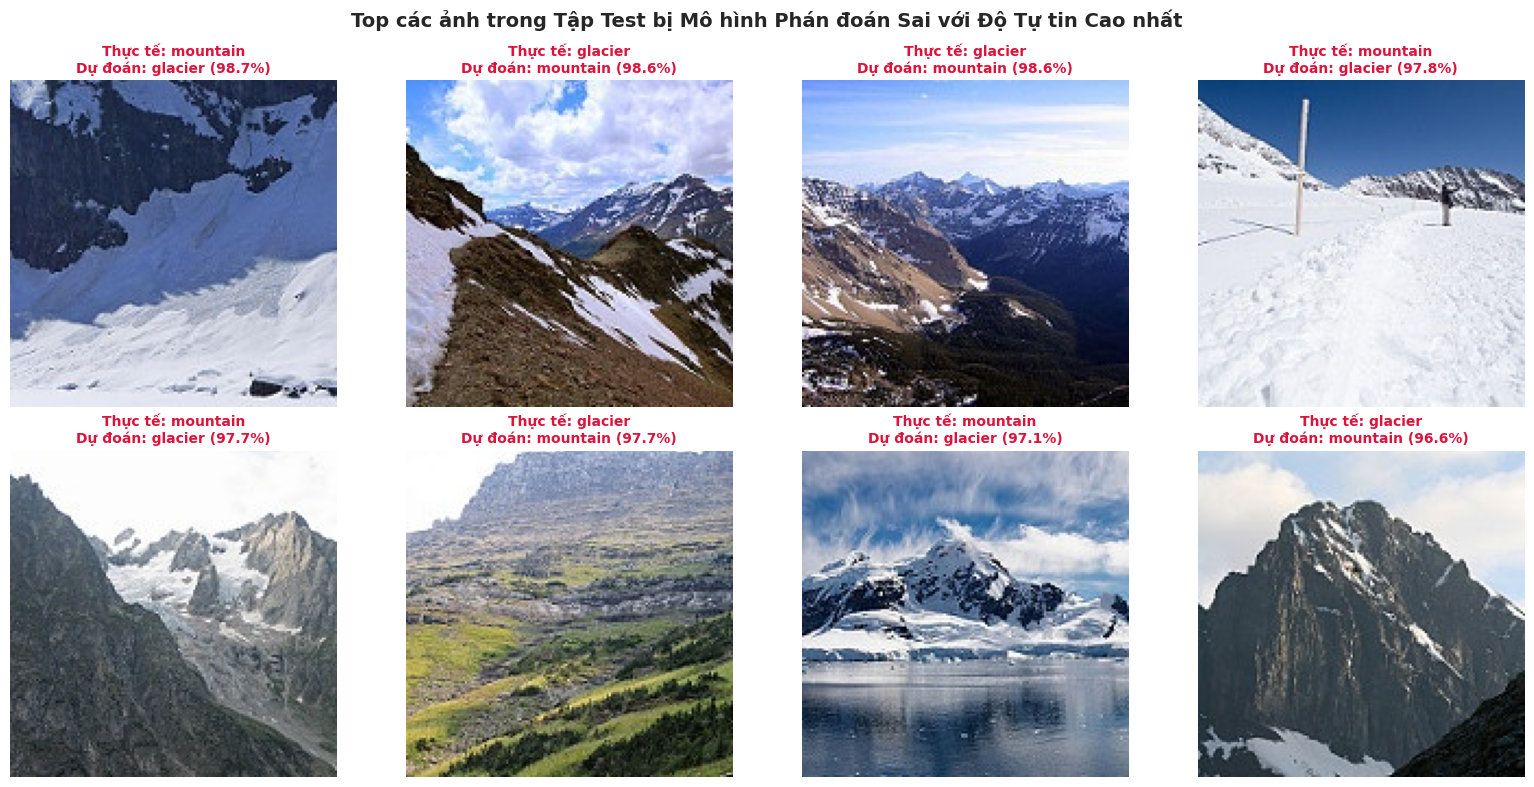
\includegraphics[width=0.88\linewidth]{image/c57_f0.png}
  \caption{Các mẫu dự đoán sai tiêu biểu của ResNet-18 (Fine-tune): nhiều ảnh chứa đồng thời cả tòa nhà và đường phố hoặc núi phủ tuyết, gây nhập nhằng ngay cả với mắt người.}
  \label{fig:img_errors}
\end{figure}

Sử dụng \textbf{Grad-CAM} (\Cref{fig:img_gradcam}) để giải thích vùng ảnh mô hình tập trung khi ra quyết định cho thấy: với các ca dự đoán đúng, \textit{ResNet-18 (Fine-tune)} định vị chính xác tán cây (\textit{forest}), mặt biển (\textit{sea}) hay mặt tiền công trình (\textit{buildings}); ngược lại ở các ca thất bại, mô hình bị phân tâm bởi vùng nền phụ (ví dụ bầu trời, sườn núi phủ tuyết hoặc dãy nhà ven đường).

\begin{figure}[H]
  \centering
  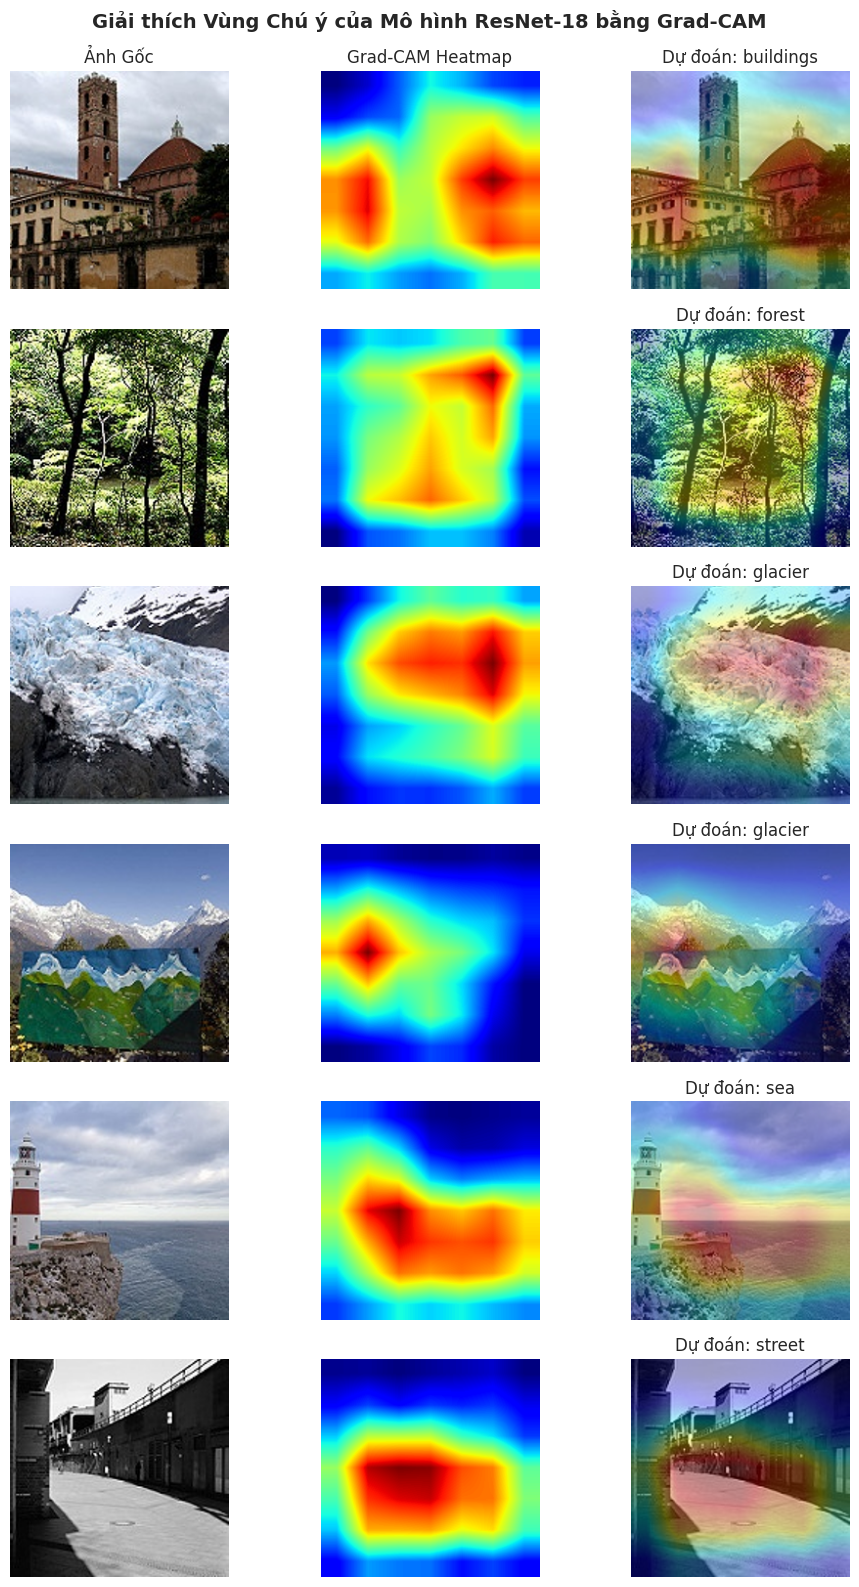
\includegraphics[width=0.88\linewidth]{image/c60_f0.png}
  \caption{Bản đồ nhiệt Grad-CAM minh họa cơ chế chú ý của ResNet-18 (Fine-tune): mô hình tập trung đúng vào đặc trưng đối tượng chính ở các mẫu dự đoán đúng và bị nhiễu nền ở các ca nhập nhằng.}
  \label{fig:img_gradcam}
\end{figure}
